\chapter{Appendix}
\label{chapter:Appendix}

\setkeys{Gin}{width=0.8\textwidth} 




\clearpage

\begin{center}
% latex table generated in R 3.0.2 by xtable 1.7-3 package
% Tue Jul 01 18:40:27 2014
\begin{table}[!h]
\centering
\begin{tabular}{|l|l|l|l|l|l|l|l|l|l|l|}
  \hline
T & cos & cos & cos & cos & cpnl & cpnl & cpnl & cpnl & cpl & cpl \\ 
  \hline
T & P & R & A & F & P & R & A & F & P & R \\ 
   \hline
0.5 & 0.65 & 0.48 & 0.50 & 0.55 & 0.63 & 0.40 & 0.46 & 0.49 & 0.67 & 0.47 \\ 
  0.6 & 0.63 & 0.32 & 0.45 & 0.42 & 0.69 & 0.21 & 0.43 & 0.32 & 0.62 & 0.33 \\ 
  0.7 & 0.65 & 0.16 & 0.41 & 0.26 & 0.60 & 0.13 & 0.39 & 0.21 & 0.67 & 0.18 \\ 
  0.8 & 0.75 & 0.10 & 0.40 & 0.17 & 0.65 & 0.08 & 0.38 & 0.15 & 0.58 & 0.10 \\ 
  0.9 & 0.71 & 0.07 & 0.39 & 0.14 & 0.71 & 0.07 & 0.39 & 0.14 & 0.71 & 0.07 \\ 
   \hline
\end{tabular}
\end{table}
% latex table generated in R 3.0.2 by xtable 1.7-3 package
% Tue Jul 01 18:40:27 2014
\begin{table}[!h]
\centering
\begin{tabular}{|l|l|l|l|l|l|l|l|l|l|l|}
  \hline
T & cpl & cpl & mih & mih & mih & mih & max & max & max & max \\ 
  \hline
T & A & F & P & R & A & F & P & R & A & F \\ 
   \hline
0.5 & 0.51 & 0.55 & 0.66 & 0.77 & 0.60 & 0.71 & 0.66 & 0.78 & 0.60 & 0.72 \\ 
  0.6 & 0.44 & 0.43 & 0.67 & 0.58 & 0.55 & 0.62 & 0.66 & 0.59 & 0.55 & 0.63 \\ 
  0.7 & 0.42 & 0.28 & 0.63 & 0.34 & 0.45 & 0.44 & 0.63 & 0.35 & 0.45 & 0.45 \\ 
  0.8 & 0.38 & 0.16 & 0.68 & 0.10 & 0.39 & 0.17 & 0.63 & 0.12 & 0.39 & 0.20 \\ 
  0.9 & 0.39 & 0.14 & 0.72 & 0.08 & 0.39 & 0.14 & 0.72 & 0.08 & 0.39 & 0.14 \\ 
   \hline
\end{tabular}
\caption{Classifier results for DBSCAN with minPts=2, epsilon=0.08 using the cluster validation strategy} 
\label{}
\end{table}\end{center}
\begin{center}
% latex table generated in R 3.0.2 by xtable 1.7-3 package
% Tue Jul 01 18:40:27 2014
\begin{table}[!h]
\centering
\begin{tabular}{|l|l|l|l|l|l|l|l|l|l|l|}
  \hline
T & cos & cos & cos & cos & cpnl & cpnl & cpnl & cpnl & cpl & cpl \\ 
  \hline
T & P & R & A & F & P & R & A & F & P & R \\ 
   \hline
0.5 & 0.72 & 0.16 & 0.41 & 0.26 & 0.70 & 0.09 & 0.39 & 0.16 & 0.72 & 0.15 \\ 
  0.6 & 0.75 & 0.07 & 0.38 & 0.12 & 0.75 & 0.04 & 0.37 & 0.07 & 0.71 & 0.07 \\ 
  0.7 & 0.81 & 0.03 & 0.37 & 0.06 & 0.80 & 0.03 & 0.37 & 0.05 & 0.81 & 0.03 \\ 
  0.8 & 0.85 & 0.02 & 0.37 & 0.04 & 0.84 & 0.02 & 0.37 & 0.04 & 0.82 & 0.02 \\ 
  0.9 & 0.85 & 0.02 & 0.37 & 0.04 & 0.85 & 0.02 & 0.37 & 0.04 & 0.85 & 0.02 \\ 
   \hline
\end{tabular}
\end{table}
% latex table generated in R 3.0.2 by xtable 1.7-3 package
% Tue Jul 01 18:40:27 2014
\begin{table}[!h]
\centering
\begin{tabular}{|l|l|l|l|l|l|l|l|l|l|l|}
  \hline
T & cpl & cpl & mih & mih & mih & mih & max & max & max & max \\ 
  \hline
T & A & F & P & R & A & F & P & R & A & F \\ 
   \hline
0.5 & 0.41 & 0.25 & 0.67 & 0.41 & 0.49 & 0.51 & 0.67 & 0.41 & 0.49 & 0.51 \\ 
  0.6 & 0.38 & 0.12 & 0.71 & 0.22 & 0.43 & 0.34 & 0.70 & 0.23 & 0.43 & 0.34 \\ 
  0.7 & 0.37 & 0.06 & 0.77 & 0.07 & 0.38 & 0.12 & 0.77 & 0.07 & 0.38 & 0.13 \\ 
  0.8 & 0.37 & 0.05 & 0.83 & 0.02 & 0.37 & 0.04 & 0.84 & 0.03 & 0.37 & 0.05 \\ 
  0.9 & 0.37 & 0.04 & 0.86 & 0.02 & 0.37 & 0.04 & 0.86 & 0.02 & 0.37 & 0.04 \\ 
   \hline
\end{tabular}
\caption{Classifier results for DBSCAN with minPts=2, epsilon=0.08 using the individual review pair validation strategy} 
\label{}
\end{table}\end{center}
\begin{center}
% latex table generated in R 3.0.2 by xtable 1.7-3 package
% Tue Jul 01 18:40:27 2014
\begin{table}[!h]
\centering
\begin{tabular}{|l|l|l|l|l|l|l|l|l|l|l|}
  \hline
T & cos & cos & cos & cos & cpnl & cpnl & cpnl & cpnl & cpl & cpl \\ 
  \hline
T & P & R & A & F & P & R & A & F & P & R \\ 
   \hline
0.5 & 0.59 & 0.39 & 0.46 & 0.47 & 0.61 & 0.33 & 0.46 & 0.43 & 0.60 & 0.39 \\ 
  0.6 & 0.66 & 0.26 & 0.46 & 0.37 & 0.60 & 0.16 & 0.42 & 0.25 & 0.61 & 0.25 \\ 
  0.7 & 0.63 & 0.15 & 0.42 & 0.24 & 0.61 & 0.13 & 0.41 & 0.22 & 0.65 & 0.16 \\ 
  0.8 & 0.71 & 0.10 & 0.42 & 0.17 & 0.64 & 0.10 & 0.41 & 0.17 & 0.57 & 0.10 \\ 
  0.9 & 0.70 & 0.09 & 0.42 & 0.17 & 0.70 & 0.09 & 0.42 & 0.17 & 0.70 & 0.09 \\ 
   \hline
\end{tabular}
\end{table}
% latex table generated in R 3.0.2 by xtable 1.7-3 package
% Tue Jul 01 18:40:27 2014
\begin{table}[!h]
\centering
\begin{tabular}{|l|l|l|l|l|l|l|l|l|l|l|}
  \hline
T & cpl & cpl & mih & mih & mih & mih & max & max & max & max \\ 
  \hline
T & A & F & P & R & A & F & P & R & A & F \\ 
   \hline
0.5 & 0.47 & 0.47 & 0.62 & 0.70 & 0.55 & 0.66 & 0.62 & 0.71 & 0.56 & 0.66 \\ 
  0.6 & 0.44 & 0.35 & 0.61 & 0.50 & 0.50 & 0.55 & 0.62 & 0.50 & 0.50 & 0.55 \\ 
  0.7 & 0.43 & 0.26 & 0.64 & 0.26 & 0.45 & 0.37 & 0.64 & 0.27 & 0.46 & 0.38 \\ 
  0.8 & 0.40 & 0.17 & 0.57 & 0.11 & 0.40 & 0.18 & 0.53 & 0.11 & 0.39 & 0.19 \\ 
  0.9 & 0.42 & 0.17 & 0.70 & 0.10 & 0.42 & 0.17 & 0.70 & 0.10 & 0.42 & 0.17 \\ 
   \hline
\end{tabular}
\caption{Classifier results for DBSCAN with minPts=2, epsilon=0.05 using the cluster validation strategy} 
\label{}
\end{table}\end{center}
\begin{center}
% latex table generated in R 3.0.2 by xtable 1.7-3 package
% Tue Jul 01 18:40:27 2014
\begin{table}[!h]
\centering
\begin{tabular}{|l|l|l|l|l|l|l|l|l|l|l|}
  \hline
T & cos & cos & cos & cos & cpnl & cpnl & cpnl & cpnl & cpl & cpl \\ 
  \hline
T & P & R & A & F & P & R & A & F & P & R \\ 
   \hline
0.5 & 0.68 & 0.14 & 0.43 & 0.23 & 0.73 & 0.08 & 0.41 & 0.15 & 0.71 & 0.14 \\ 
  0.6 & 0.79 & 0.06 & 0.41 & 0.12 & 0.75 & 0.03 & 0.40 & 0.07 & 0.76 & 0.06 \\ 
  0.7 & 0.84 & 0.03 & 0.40 & 0.06 & 0.82 & 0.03 & 0.39 & 0.05 & 0.84 & 0.03 \\ 
  0.8 & 0.85 & 0.02 & 0.39 & 0.05 & 0.83 & 0.02 & 0.39 & 0.04 & 0.81 & 0.02 \\ 
  0.9 & 0.85 & 0.02 & 0.39 & 0.04 & 0.85 & 0.02 & 0.39 & 0.04 & 0.85 & 0.02 \\ 
   \hline
\end{tabular}
\end{table}
% latex table generated in R 3.0.2 by xtable 1.7-3 package
% Tue Jul 01 18:40:27 2014
\begin{table}[!h]
\centering
\begin{tabular}{|l|l|l|l|l|l|l|l|l|l|l|}
  \hline
T & cpl & cpl & mih & mih & mih & mih & max & max & max & max \\ 
  \hline
T & A & F & P & R & A & F & P & R & A & F \\ 
   \hline
0.5 & 0.43 & 0.23 & 0.64 & 0.39 & 0.49 & 0.49 & 0.64 & 0.40 & 0.49 & 0.49 \\ 
  0.6 & 0.41 & 0.11 & 0.69 & 0.21 & 0.45 & 0.32 & 0.69 & 0.21 & 0.45 & 0.32 \\ 
  0.7 & 0.40 & 0.07 & 0.76 & 0.05 & 0.40 & 0.10 & 0.76 & 0.06 & 0.40 & 0.11 \\ 
  0.8 & 0.39 & 0.05 & 0.80 & 0.02 & 0.39 & 0.05 & 0.81 & 0.03 & 0.39 & 0.05 \\ 
  0.9 & 0.39 & 0.04 & 0.86 & 0.02 & 0.39 & 0.04 & 0.86 & 0.02 & 0.39 & 0.04 \\ 
   \hline
\end{tabular}
\caption{Classifier results for DBSCAN with minPts=2, epsilon=0.05 using the individual review pair validation strategy} 
\label{}
\end{table}\end{center}

\clearpage

\begin{table}
\begin{center}
    \begin{tabular}{ | p{0.3\textwidth} | p{0.2\textwidth} |}
    \hline
    \textbf{Word} & \textbf{Frequency} \\ \hline
      delivery & 1086\\ \hline
	company & 1148\\ \hline
	website & 1154\\ \hline
	customer & 1209\\ \hline
	recommend & 1737\\ \hline
	time & 1787\\ \hline
	buy & 1788\\ \hline
	good & 1918\\ \hline
	great & 1940\\ \hline
	order & 2069\\ \hline
	price & 2085\\ \hline
	service & 2563\\ \hline
	number & 2872 \\ \hline
    \end{tabular}
\caption{Word frequencies in the Trustpilot review dataset}
\label{tab:wordfreq}
\end{center}
\end{table}

\begin{figure}
\begin{center}
\subfloat[Subfigure 1 list of figures text][all words]{
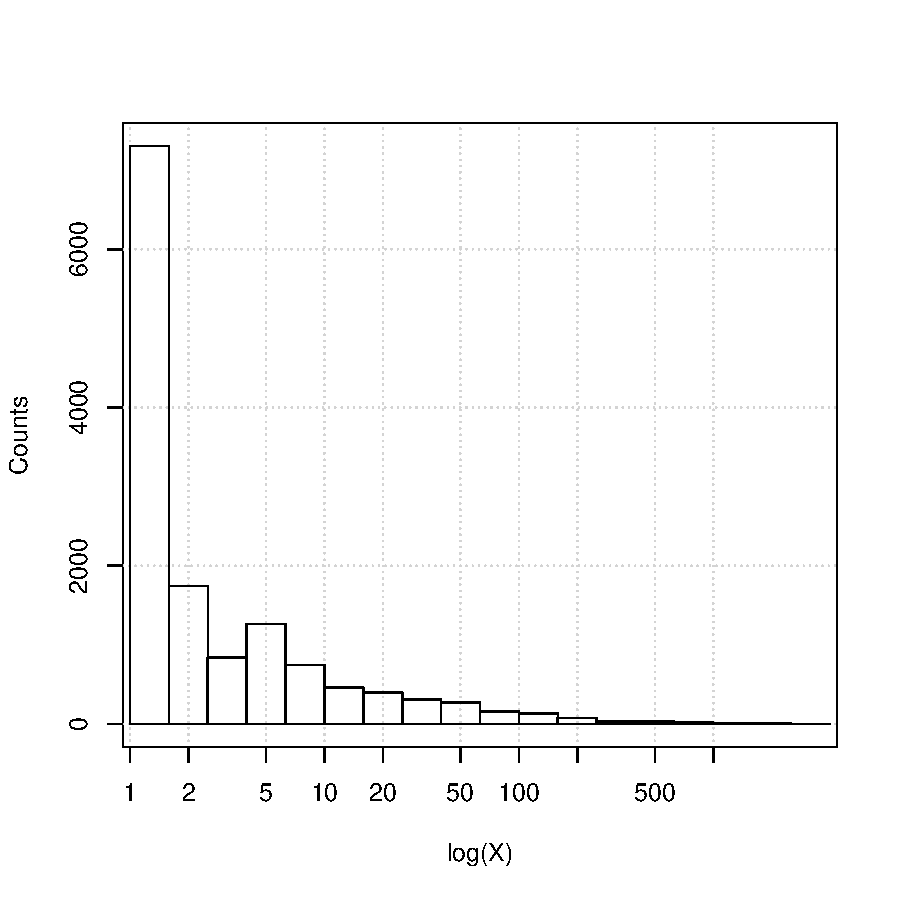
\includegraphics[width=0.5\textwidth]{sweave/sweave-lda-words-all-hist}
\label{fig:lda-words-all-hist-appendix}}
\subfloat[Subfigure 2 list of figures text][words with a frequency between 5 and 100]{
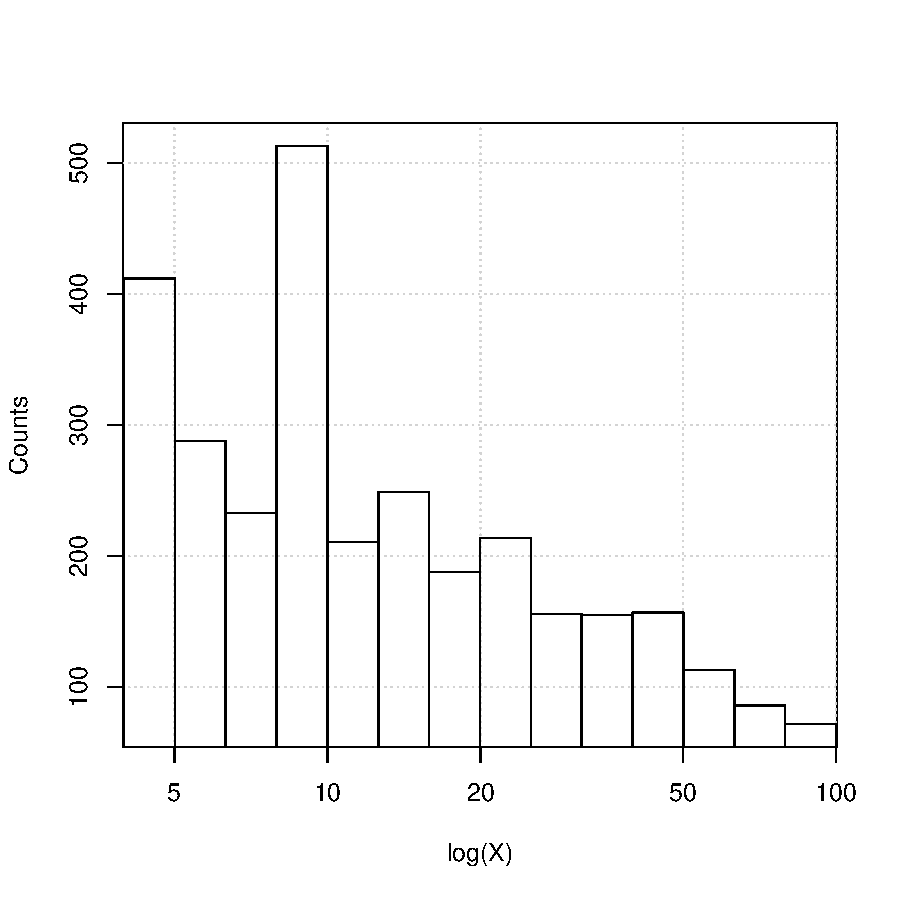
\includegraphics[width=0.5\textwidth]{sweave/sweave-lda-words-5-100-hist}
\label{fig:lda-words-5-100-hist-appendix}}
\qquad
\caption{Log histogram for the words' frequencies}    
\label{fig:lda-words-hist-5-100-appendix}
\end{center}
\end{figure}

\begin{figure}[ht]
\begin{center}
\subfloat[Subfigure 1 list of figures text][Precision]{
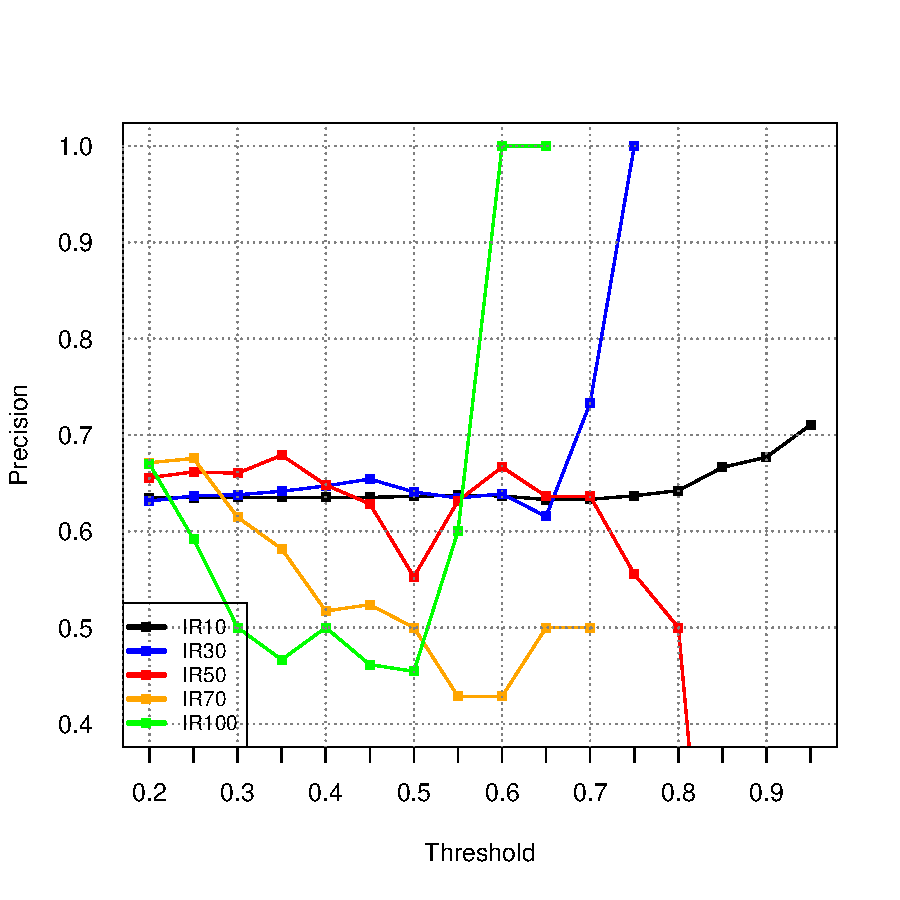
\includegraphics[width=0.5\textwidth]{sweave/sweave-lda-precision-all-words}
\label{fig:lda_precision-appendix}}
\subfloat[Subfigure 2 list of figures text][Recall]{
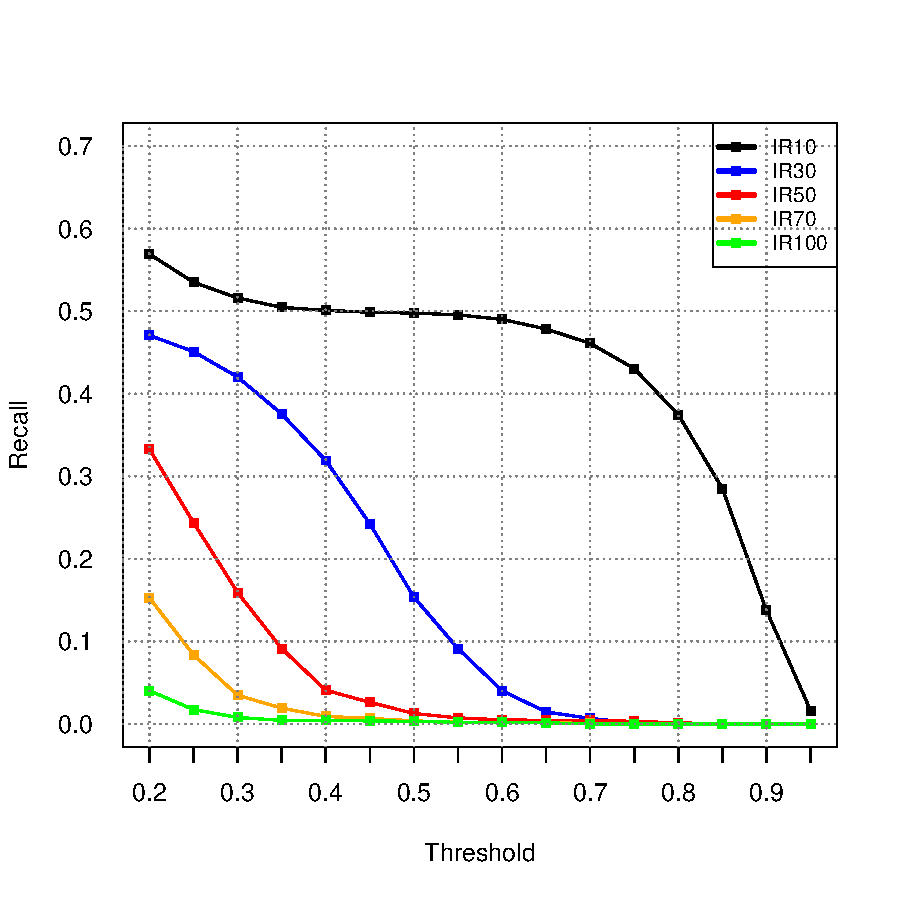
\includegraphics[width=0.5\textwidth]{sweave/sweave-lda-recall-all-words}
\label{fig:lda_recall-appendix}}
\qquad
\begin{center}
\subfloat[Subfigure 3 list of figures text][F1 Score]{
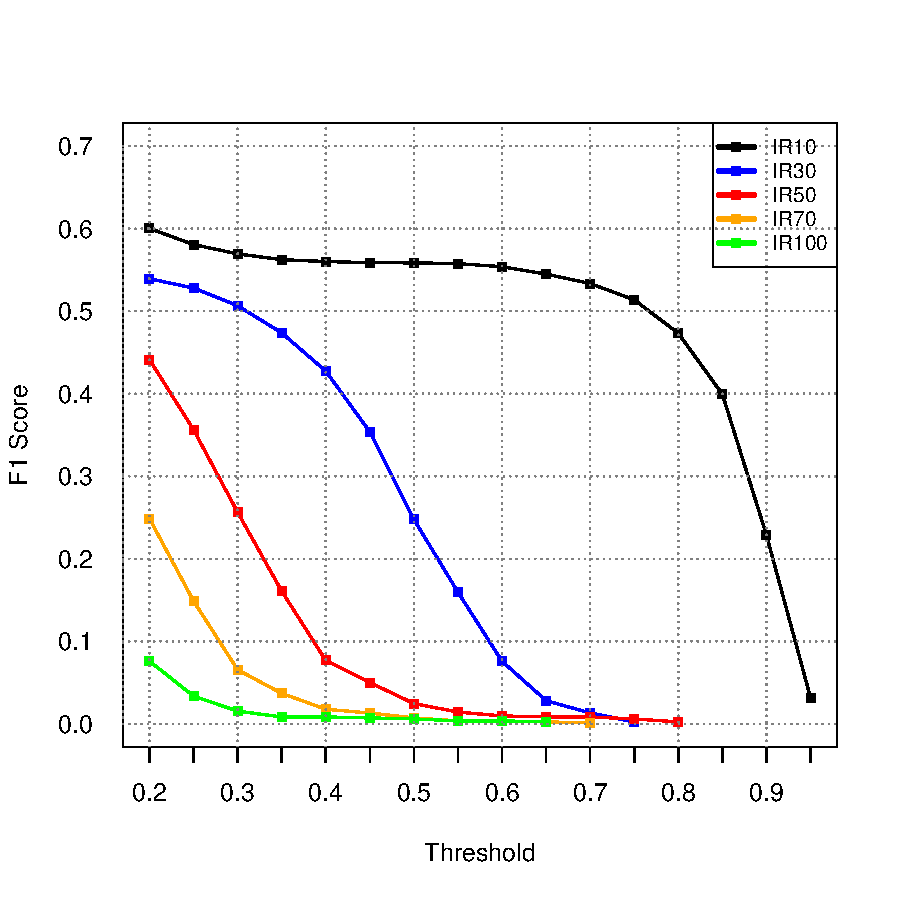
\includegraphics[width=0.5\textwidth]{sweave/sweave-lda-f1score-all-words}
\label{fig:lda_f1score-appendix}}
\end{center}
\caption{LDA results for the information radius similarity measure for all words regardless of their frequency}    
\label{fig:lda-appendix-all-words}
\end{center}
\end{figure}

\begin{figure}[ht]
\begin{center}
\subfloat[Subfigure 1 list of figures text][Precision]{
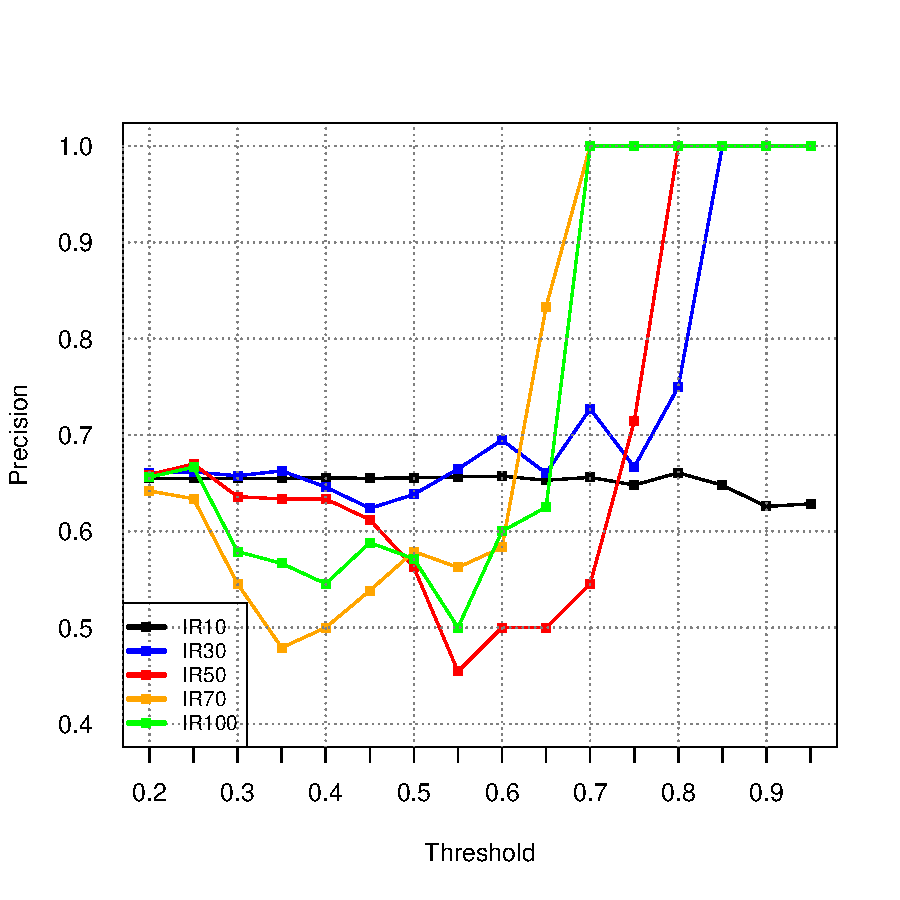
\includegraphics[width=0.5\textwidth]{sweave/sweave-lda-precision-5-100-words}
\label{fig:lda_precision-appendix}}
\subfloat[Subfigure 2 list of figures text][Recall]{
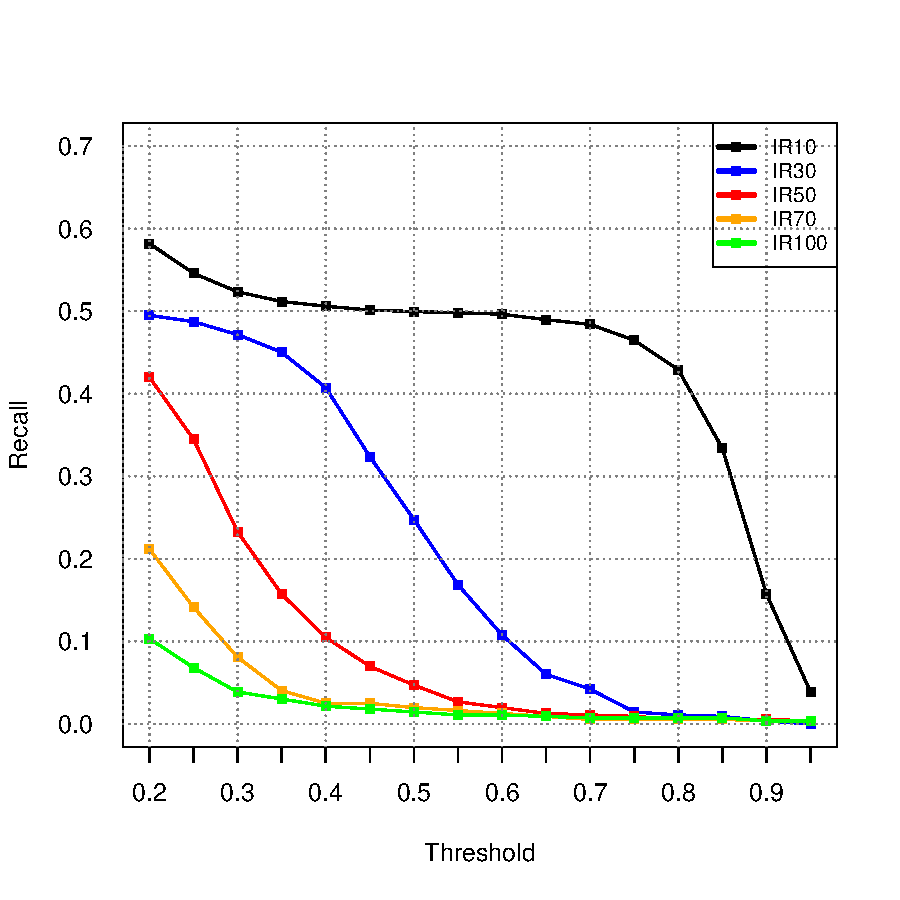
\includegraphics[width=0.5\textwidth]{sweave/sweave-lda-recall-5-100-words}
\label{fig:lda_recall-appendix}}
\qquad
\begin{center}
\subfloat[Subfigure 3 list of figures text][F1 Score]{
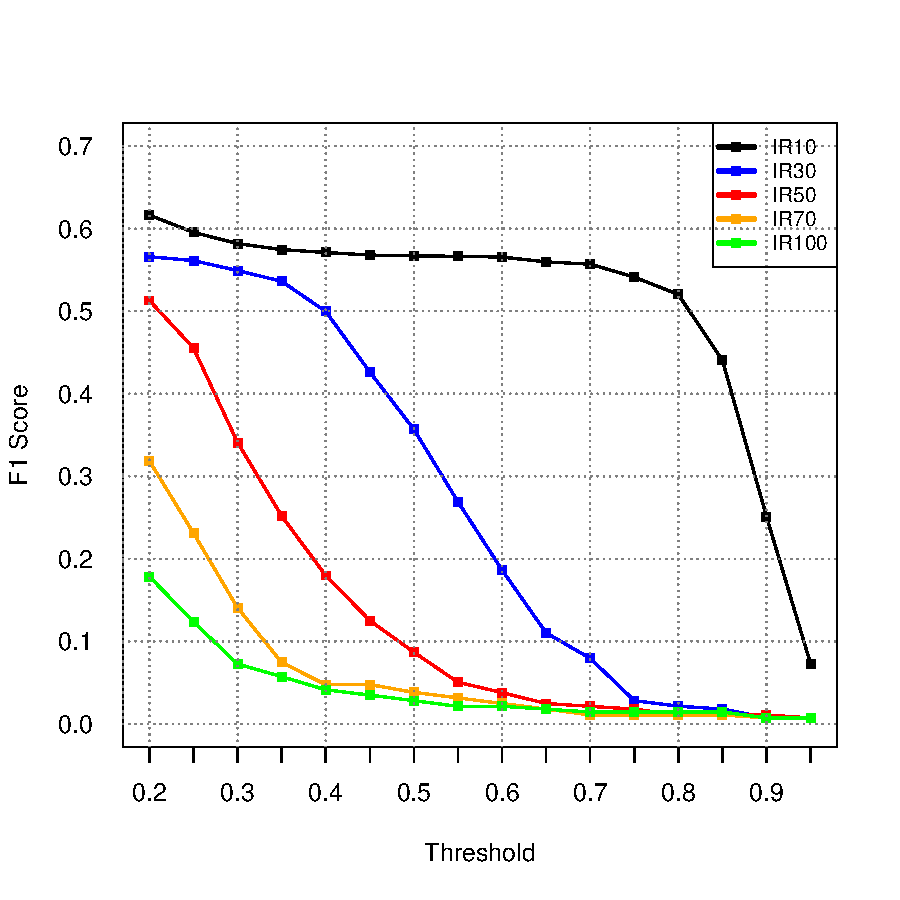
\includegraphics[width=0.5\textwidth]{sweave/sweave-lda-f1score-5-100-words}
\label{fig:lda_f1score-appendix}}
\end{center}
\caption{LDA results for the information radius similarity measure for words with a frequency between 5 and 100}    
\label{fig:lda-appendix-5-100-words}
\end{center}
\end{figure}
